\subsection{Formulation d'une réponse à partir de l'information d'intérêt retenue}

Bien qu’il est intéressant de trouver l’endroit où porter attention dans un corpus textuel, il est tout autant intéressant de savoir comment générer une réponse structurée et concise à l’utilisateur. Cela peut être fait en utilisant le \gls{hred} tel qu’introduit par \cite{chatbot\string:HRED}. En effet, \gls{hred} est une imbrication hiérarchique de réseaux de neurones récurrents. Un premier est utilisé afin d’encoder les phrases, un second est nécessaire afin de garder le contexte des réponses passées lesquelles ont déjà été traitées \footnote{Comme un suivi de la discussion dans une mémoire temporaire} et un troisième \gls{rnn} est mis à profit afin de décoder l’information en une réponse à l’utilisateur. En adaptant l'architecture neurale \gls{hred} de façon à lui donner des mécanismes d'attention tels que précédemment expliqués, il est possible de générer la réponse en retour de la requête attentionnelle à l’utilisateur. Ainsi, en ayant le contexte de la question que l'utilisateur pose ainsi que le contexte des documents à parcourir avec les mécanismes d’attention, il est possible de chercher dans le texte ce qu'il faut comme information, ce qui est envoyé au décodeur du \gls{hred} lequel peut répondre avec le nouveau contexte de l'information trouvée par la recherche effectuée. Ainsi, le premier \gls{rnn} du \gls{hred} qui encode l’information peut utiliser \texttt{word2vec} \cite{word2vec} directement, en plus de l'\textit{embedding} provenant de l’avant dernière couche de neurones du \gls{dnn} de la partie \gls{stt}. En plus de cela, il est possible d’utiliser \texttt{inferSent} de \textbf{Facebook} \cite{inferSent}, dont la sortie pourra être concaténée au signal de sortie du \gls{rnn} encodeur du \gls{hred}, en tant qu'\textit{embedding} supplémentaire au niveau des phrases plutôt qu’au niveau des mots comme expliqué à la \autoref{devel:embedding}. \\

Dans une amélioration plus récente de l’architecture \gls{hred} \cite{chatbot\string:LVHRED}, présentée à la \autoref{fig:lvHred}, il est possible d’utiliser une variable latente intermédiaire laquelle permet de faire le pont entre les réponses envoyées du décodeur vers l’utilisateur, en plus de réinjécter cette réponse dans l’encodeur qui écoute la réponse de l’utilisateur après lui avoir répondu une première fois. En retournant ainsi l'information du décodeur dans l’encodeur, le contexte se retrouve à être conservé d’une phrase à la prochaine et d'ainsi avoir un discours plus fluide tout en étant moins assujettis à des variations subites de sujet ou d'interprétation. D'autre part, ce passage d'information aura pour effet de renforcer la qualité de la requête attentionnelle laquelle peut être générée à la toute fin de l’encodeur du \gls{hred}. C'est à ce moment que le mécanisme d’attention décrit dans la \autoref{devel:qa} portant sur l’analyse de texte suite à des questions pourrait être inséré. Une fois la question posée par l’utilisateur et lue dans l’encodeur, le \gls{hred} peut bénéficier de cette question dans son \gls{rnn} intermédiaire, et ce, en tant que requête attentionnelle à passer directement au système attentionnel. Des travaux similaires ont été réalisés par \cite{readNcomprehend}, chez \textbf{Google}. Somme toutes, le \gls{hred} aura accès à la question de l’utilisateur et au corpus de texte dans lequel il peut maintenant cibler l’information pertinente.

\begin{figure*}
  \centering
  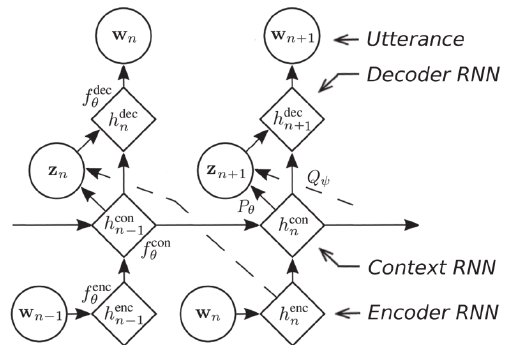
\includegraphics[width=\textwidth]{lvHred}
  \caption{L'architecture \gls{hred} améliorée avec une variable latente \cite{chatbot\string:LVHRED}}
  \label{fig:lvHred}
\end{figure*}

Étant donné la taille énorme du corpus textuel dans lequel le réseaux de neurones peut lire l’information \footnote{L’ensemble du texte sur Wikipédia par exemple}, il est possible d’appliquer un \texttt{MapReduce} \cite{DeanMapReduce} pour ainsi améliorer les performances de ce processus et réduire de façon importante le temps de réponse de notre assistant, ce qui est un aspect primordial à son déploiement et son adoption de la part de l'utilisateur. Cette technique procède de façon distribuée sur plusieurs centaines d’ordinateurs. Dans le cas présent, ceux-ci utiliseraient eux-même les implémentations de \texttt{word2vec} et de \texttt{inferSent} sur le corpus d'information, et cela en ayant en main la requête attentionnelle générée par le mécanisme d'attention, selon les principes de \texttt{MapReduce}. Cette partie, qui est distribuée et qui est surnommée, le lecteur impatient, est exposée à la \autoref{fig:teachingImpatientReader}. Il existe même une amélioration possible sur cet architecture neurale. Il est visible dans la figure que plusieurs itérations entre la requête et le système attentionnel est fait. Cela devrait être simplifié en une seule étape afin de réduire la complexité algorithmique de linéaire à constante en fonction de la longueur de la requête, en termes de nombre de mots. La recherche suivant la requête pouvant être distribuée, il devient donc très rapide d'accomplir le celle-ci, tout comme l'ensemble des opérations décrites aux sections précédentes.

\begin{figure*}
  \centering
  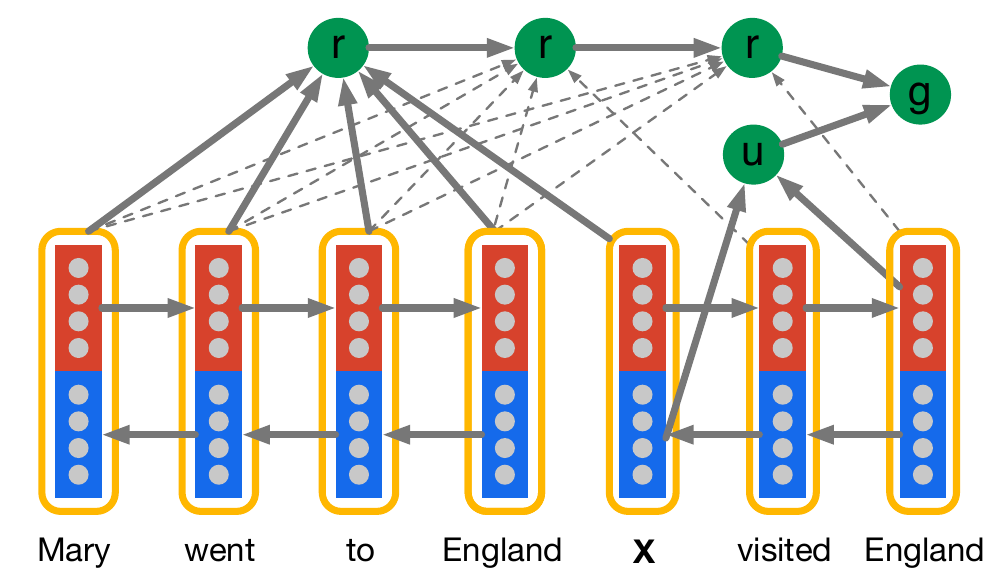
\includegraphics[width=\textwidth]{teachingImpatientReader}
  \caption{Le lecteur impatient prends la requête \textit{X visited England} afin de faire une recherche dans le texte \textit{Mary went to England}, à l’aide du mécanisme d’attention lequel est ici dénoté \texttt{r}, assisté de la requête \texttt{u} \cite{readNcomprehend}}
  \label{fig:teachingImpatientReader}
\end{figure*}
